\chapter{Aerial Robotics}
\section{Introduction}
The field of \textit{Aerial Robotics} has become a new frontier of Field Robotics; its main focus is the study of robotic systems capable of flight. It is easy to see how such systems could be of great help in many fields, going from aerial exploration of disaster zones, transportation, maintenance of infrastructure, logistics. There is a wide variety of aerial robots, classified by many metrics; for example, either by their level of autonomy:
\begin{itemize}
    \item UAV: \textit{Unmanned Aerial Vehicle}.
    \item UAS: \textit{Unmanned Aerial System}.
    \item RPV: \textit{Remotely Piloted System}.
    \item ROA: \textit{Remotely Operated Aircraft}.
    \item UVS: \textit{Unmanned Vehicle System}.
\end{itemize}
Or by the flying apparatus:
\begin{itemize}
    \item \textit{Fixed-wing}.
    \item \textit{Rotary-wing}.
    \item \textit{Tilted}, \textit{Tilting} configurations.
    \item \textit{Flapping wings}.
\end{itemize}
Aerial robots can also be distinguished by their highest reachable altitude, physical dimension, ecc. A recent development in this field has been \textit{Aerial Manipulation}: an aerial robot with a manipulator mounted on its chassis. 
\section{Dynamic Models}
\subsection{Introduction: Reference Frames}
Aerial Robots are very much different from wheeled ones; in fact, this difference also extends to the Frames of Reference used to localize the robot. 
\begin{figure}[htbp!]
    \begin{minipage}{0.4\textwidth}
        In the \textit{Earth Centered Inertial Frame} the frame's origin is Earth's center and the axes orientations are fixed, such that the $xy$-plane contains the Equator; the $z$-axis is positive in the direction of the North Pole.
    \end{minipage} \hfill
    \begin{minipage}{0.6\textwidth}
        \centering
        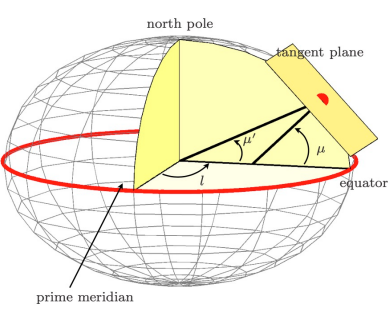
\includegraphics[width=0.6\linewidth]{Images/image27.png}
        \caption{Earth Centered Inertial FoR.}
        \label{fig:earth_centered_inertial_for}
    \end{minipage}\vfill
    \begin{minipage}{0.4\textwidth}
        The \textit{Earth Centered Earth-Fixed Frame} is mostly the same of the ECI, with the difference that the axes are moving with the Earth so that this is a non-inertial frame. GPS gives position with respect to this FoR.
    \end{minipage}\hfill
    \begin{minipage}{0.6\textwidth}
        \centering
        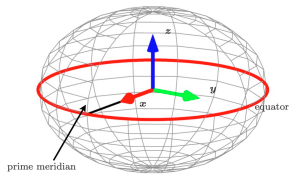
\includegraphics[width=0.6\linewidth]{Images/image28.png}
        \caption{Earth Centered Non-Inertial FoR.}
        \label{fig:earth_centered_non_inertial_for}
    \end{minipage}\vfill
    \begin{minipage}{0.4\textwidth}
        In the \textit{North-East-Down} frame the Frame of Reference is attached to a tangent plane to the Earth and is only a local description limited to the area of interest. Notice that the $z$-axis points down; the same frame of reference, but with the $z$-axis point away from the Earth's center, is called \textit{East-North-Up}.
    \end{minipage}\hfill
    \begin{minipage}{0.6\textwidth}
        \centering
        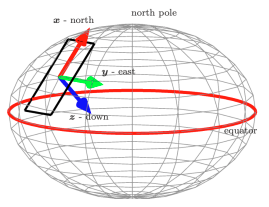
\includegraphics[width=0.6\linewidth]{Images/image29.png}
        \caption{\textit{North-East-Down} FoR.}
        \label{fig:NED_for}
    \end{minipage}
\end{figure}\\
The usual \textit{Latitude-Longitude-Altitude} or \textit{Geographic Latitude} are also used.       
\begin{figure}[htbp!]
    \begin{minipage}{0.4\textwidth}
        \centering
        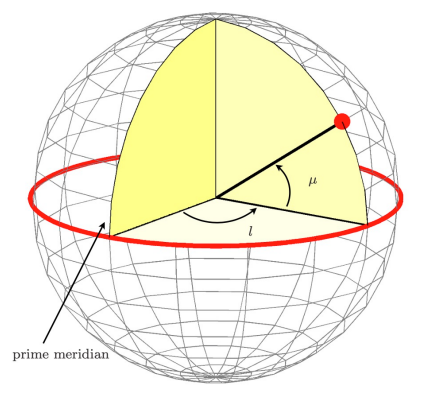
\includegraphics[width=0.4\linewidth]{Images/image30.png}
        \caption{\textit{Latitude-Longitude-Altitude} FoR.}
        \label{fig:latitude_longitude_altitude_for}
    \end{minipage} \hfill
    \begin{minipage}{0.4\textwidth}
        \centering
        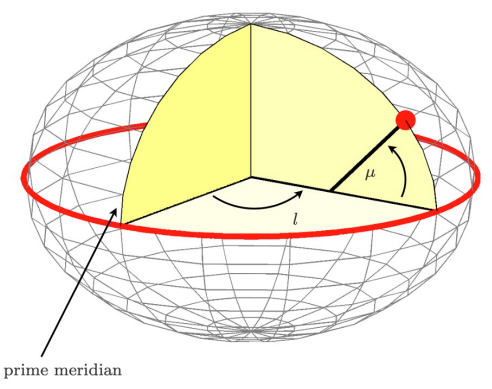
\includegraphics[width=0.4\linewidth]{Images/image31.png}
        \caption{\textit{Geographic Latitude} FoR.}
        \label{fig:geographic_latitude_for}
    \end{minipage}\vfill
\end{figure}
\subsection{Inputs}
The actuation units are mechatronic components producing thrust which typically consist of a brushless motor with a single propeller, attached to the main body either rigidly or through a mechatronic system comprising other joints and servomotors (e.g., tilted/tilting actuation units).
\begin{figure}[htbp!]
    \begin{minipage}{0.6\textwidth}
        \centering
        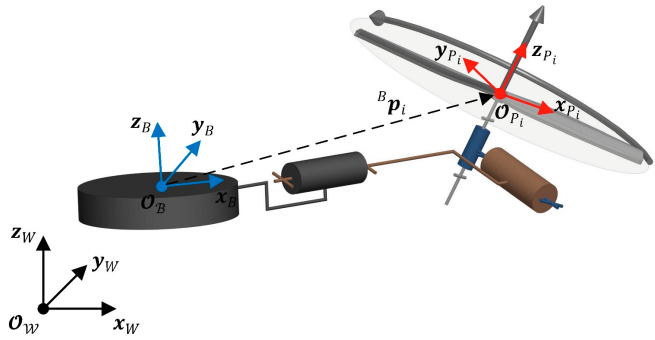
\includegraphics[width=0.6\linewidth]{Images/image33.png}
        \caption{World and Propeller Frame.}
    \end{minipage}\hfill
    \begin{minipage}{0.4\textwidth}
        For each propeller, define a frame rigidly attached to the brushless motor (not spinning with the propeller), whose position w.r.t. the body frame is given as $p_i^b$, $i\in\{1,\dots,n\}$; define the rotation axis of each motor as $z_{P_i}^{b}$. Notice that in tilting configurations (such as the one in the picture) this FoR can change its orientation, which is then given by $R_{P_i}^{b}(\alpha_i,\beta_i)\in SO(3)$, where $\alpha_i,\beta_i$ are radial and tangential rotation angles.
    \end{minipage} 
\end{figure}\\
Each propeller causes thrust and drag forces, the latter due to air resistance opposing the propeller's blades rotation. The rotation of the propeller also causes an angular momentum on the UAV's body, this is the reason why opposing propellers rotate in opposite directions: the net momentum is zero. Let us neglect:
\begin{itemize}
    \item The effects due to the propeller inertia.
    \item Flapping effects and other aerodynamic effects.
\end{itemize}
And also suppose that:
\begin{itemize}
    \item The UAV is far from obstacles. 
    \item The UAV is in a quasi-static regime (i.e. very slow).
\end{itemize}
Then, both thrust and drag can be modelled as:
\begin{equation}\label{thrust_drag_model}
    \begin{cases}
        f_{P_i}=k_{f}|\omega_i|\omega_i \\
        m_{P_i}=k_i k_{m}|\omega_i|\omega_i
    \end{cases}
\end{equation}
Where $k_{f},k_{m}>0$ are the thrust and drag factors, $k_i=1,k_i=-1$ for a descending or ascending chord, respectively. The total thrust and torque on the UAV's body is then obtained by summation:
\begin{gather*}
    f^b=\sum_{i=1}^{n}{k_{f}|\omega_i|\omega_iz_{P_i}^b}\\
    \tau^b=\sum_{i=1}^{n}{|\omega_i|\omega_i\left(-k_ik_{m}z_{P_i}^{b}+k_{f}S\left(p_{P_i}^b\right)z_{P_i}^{b}\right)}
\end{gather*}
Besides, assuming that the brushless motor are velocity controlled, it is possible to define $u_{\omega_i}=|\omega_i|\omega_i\in\mathbb{R}$ as one of the controllable inputs for the $i$-th propeller. Since it is possible to write:
\begin{equation*}
    \begin{bmatrix}
        f^b \\ \tau^b
    \end{bmatrix}=f_u(\alpha_i,\beta_i,u_{\omega_i})
\end{equation*}
The inputs are mapped from the velocity inputs $u_{\omega_i}$ by the \textit{Allocation Matrix}.
\begin{definition}\label{Allocation_Matrix}
    (\textit{Allocation Matrix}): The allocation matrix is the map $G_q:\mathbb{R}^{m_1}\rightarrow\mathbb{R}^{m_2}$, mapping the velocity inputs $u_{\omega_i}$, $i\in\{1,\dots,m_1\}$ to the vector of forces and torques $\begin{bmatrix}f^b & \tau^b\end{bmatrix}^{T}$.
\end{definition}
As an example, for a nontilting quadcopter, the allocation matrix is:
\begin{equation*}
    \begin{bmatrix}
        f_x \\ f_y \\ f_z \\ \tau_x \\ \tau_y \\ \tau_z
    \end{bmatrix}=
    \begin{bmatrix}
        0 & 0 & 0 & 0\\
        0 & 0 & 0 & 0\\
        -k_{f} & -k_{f} & -k_{f} & -k_{f}\\
        0 & -lc_f & 0 & -lc_f\\
        -k_{m} & k_{m} & -k_{m} & k_{m}
    \end{bmatrix}
    \begin{bmatrix}
        u_{\omega_1} \\ u_{\omega_2} \\ u_{\omega_3} \\ u_{\omega_4}
    \end{bmatrix}
\end{equation*}
Notice that:
\begin{itemize}
    \item Given the two null rows of the Allocation Matrix, the quadcopter is an underactuated system (the map $\dot{x}=f_u(x,u)$ is not surjective, since the nullspace of $G_q$ is not trivial).
    \item To avoid the underactuation, meaning that $G_q\in\mathbb{R}^{6\times n}$ is full column-rank, either non coplanar propellers (\textit{tilted configuration} UAVs) or motorized propellers (\textit{actively tilting configurations}) should be used.
\end{itemize}
\newpage
\subsection{Dynamic Models: non-tilting UAVs}
\begin{figure}[htbp!]
    \begin{minipage}{0.5\textwidth}
        Consider two reference frames, a \textit{Body-Fixed} frame (NED) and a \textit{World-Fixed} frame (also NED), such as in the picture. The pose of the robot can be represented by the usual position vector and rotation matrix. Assuming that the attitude has been expressed by the Euler Angles minimal representation.
    \end{minipage} \hfill
    \begin{minipage}{0.6\textwidth}
        \centering
        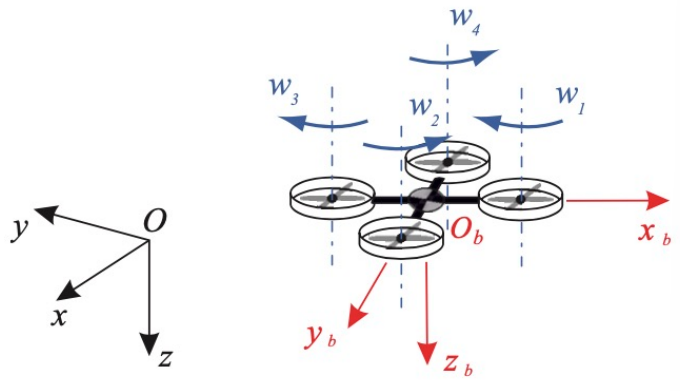
\includegraphics[width=0.6\linewidth]{Images/image32.png}
        \caption{Body and World FoR.}
    \end{minipage}
\end{figure}
\begin{gather*}
    p_b=\begin{bmatrix}
        x & y & z
    \end{bmatrix}^{T} \\
    R_b = \begin{bmatrix}
        x_b & y_b & z_b
    \end{bmatrix}\in SO(3), \\
    R_b(\eta_b)=\begin{bmatrix}
        c_{\theta}c_{\psi} & s_{\phi}s_{\theta}c_{\psi}-c_{\phi}s_{\psi} & c_{\phi}s_{\theta}c_{\psi}+s_{\phi}s_{\psi} \\
        c_{\theta}s_{\psi} & s_{\phi}s_{\theta}s_{\psi}+c_{\phi}c_{\psi} & c_{\phi}s_{\theta}s_{\psi}-s_{\phi}c_{\psi}\\
        -s_{\theta} & s_{\phi}c_{\theta} & c_{\phi}c_{\theta}
    \end{bmatrix}
\end{gather*}
Then, the dynamic model can be written with respect to the Body Frame as:
\begin{definition}\label{UAV_dyn_model_def}
    (\textit{UAV Dynamic Model}):
    \begin{equation}
        \begin{cases}\label{UAV_dyn_model}
            m\ddot{p}_{b}^{b}=-mS\left(\omega_{b}^{b}\right)\dot{p}_{b}^{b}+mgR_{b}^{T}e_{3}+f^b+f_{e}^b\\
            \dot{R}_{b}=R_{b}S\left(\omega_b^b\right)\\
            J_{b}\dot{\omega}_{b}^{b}=-S\left(\omega_b^b\right)J_{b}\omega_{b}^{b}+\tau^b+\tau_{e}^b
        \end{cases}
    \end{equation}
    Where:
    \begin{itemize}
        \item $e_3=\begin{bmatrix} 0 & 0 & 1\end{bmatrix}^{T}$\\
        \item $I_b\in\mathbb{R}^{3\times 3}$ is the diagonal inertia matrix of the body.
        \item $g$ is the constant vector of gravitational acceleration.
        \item $f_{e}^{b},\tau_{e}^{b}\in\mathbb{R}^{r}$ are external or unmodelled terms expressed in the body frame.
        \item $f_b= \begin{bmatrix}f_x & f_y & f_z \end{bmatrix}$.
        \item $\tau_b= \begin{bmatrix}\tau_x & \tau_y & \tau_z \end{bmatrix}$.
    \end{itemize}
\end{definition}
However, in terms of control systems a great simplification comes from expressing the linear motion with respect to the World Frame; by recalling that:
\begin{gather*}
    \dot{p}_b=R_b\dot{p}_{b}^{b}\rightarrow \ddot{p}_{b}=R_b\ddot{p}_{b}^{b}+R_bS\left(\omega_{b}^{b}\right)\dot{p}_{b}^{b}\
\end{gather*}
Multiplying both sides of the linear dynamics by $R_b$ and substituting:
\begin{gather*}
    mR_b\ddot{p}_b^b=-mR_bS\left(\omega_b^b\right)\dot{p}_b^b+mgR_bR_b^Te_3+R_bf^b+R_bf_e^b\rightarrow\\
    m\left(\ddot{p}_b-R_bS\left(\omega_b^b\right)\dot{p}_b^b\right)=mR_bS\left(\omega_b^b\right)\dot{p}_b^b+mgR_bR_b^Te_3+R_bf^b+R_bf_e^b
\end{gather*}
The \textit{Geometric Dynamic Model} for an UAV is obtained.
\begin{definition}\label{UAV_geomtric_dyn_model_def}
    (\textit{Geometric Dynamic Model} of an UAV):
    \begin{gather}\label{UAV_geomtric_dyn_model}
        \begin{cases}
            m\ddot{p}_b=mge_3+R_bf^b+f_e\\
            \dot{R}_b=R_bS\left(\omega_b^b\right)\\
            I_b\dot{\omega}_b^b=-S\left(\omega_b^b\right)I_b\omega_b^b+\tau^b+\tau_e^b
        \end{cases}
    \end{gather}
\end{definition}
Lastly, the model can be formulated with respect to the Euler's Angles; notice that:
\begin{equation*}
    \omega_b^b=Q(\eta_b)\dot{\eta}_b\rightarrow\ddot{\eta}_b=\dot{Q}^{-1}\omega_b^b+Q^{-1}\dot{\omega}_b^b
\end{equation*}
Provided that $\theta\neq\pm\pi/2$. The idea is to replace the coordinate-free quadrotor dynamic model to the vector $\dot{\omega}_b^b$:
\begin{gather*}
    \ddot{\eta}_b=\dot{Q}^{-1}\omega_b^b+Q^{-1}\dot{\omega}_b^b\rightarrow\\
    \ddot{\eta}_b=\dot{Q}^{-1}\omega_b^b+Q^{-1}\left[-S\left(\omega_b^b\right)I_b\omega_b^b+\tau^b+\tau_e^b\right] \rightarrow \\
    \left\{Q^{T}I_bQ\right\}\ddot{\eta}_b=\left\{Q^{T}I_bQ\right\}\dot{Q}^{-1}\omega_b^b+\left\{Q^{T}I_bQ\right\}Q^{-1}\left[-S\left(\omega_b^b\right)I_b\omega_b^b+\tau^b+\tau_e^b\right] \rightarrow \\
\end{gather*}
Since $\dot{Q}=-Q\dot{Q}^{-1}Q\rightarrow\dot{Q}^{-1}Q=-Q^{-1}\dot{Q}$ holds, it follows and defining $M\left(\eta_b\right)=\left\{Q^{T}I_bQ\right\}$:
\begin{gather*}
    M\left(\eta_b\right)\ddot{\eta}_b=Q^{T}I_b\dot{Q}\dot{\eta}_b+Q^{T}\left[-S\left(Q\dot{\eta}_b\right)I_bQ\dot{\eta}_b+\tau^b+\tau_e^b\right]
\end{gather*}
Then, the \textit{RPY dynamic model} is obtained.
\begin{definition}\label{UAV_RPY_dyn_model_def}
    (\textit{RPY dynamic model} of an UAV):
    \begin{equation}\label{UAV_RPY_dyn_model}
        \begin{cases}
            m\ddot{p}_b=mge_3+R_bf^b+f_e\\
            M(\eta_b)\ddot{\eta}_b=-C(\eta_n,\dot{\eta}_b)\dot{\eta}_b+Q^{T}(\eta_b)\tau^b+Q^{T}(\eta_b)\tau_e^b
        \end{cases}
    \end{equation}
    Where:
    \begin{itemize}
        \item $M(\eta_b)=Q^{T}(\eta_b)I_bQ(\eta_b)\in\mathbb{R}^{3\times 3}$ is symmetric and positive definite, provided that $\theta=\pm\pi/2$.
        \item $C(\eta_b,\dot{\eta}_b)=Q^{T}(\eta_b)\cdot S(Q(\eta_b)\dot{\eta}_b)\cdot I_b \cdot Q(\eta_b)+Q^{T}(\eta_b)\cdot I_b\cdot \dot{Q}(\eta_b) \in \mathbb{R}^{3\times 3}$ and $S(\cdot )\in \mathbb{R}^{3\times 3}$ is the skew-symmetric operator representing vector product.
        \item $Q(\eta_b)\in\mathbb{R}^{3\times 3}$ is the transformation matrix such that $\omega_b^b=Q(\eta_b)\dot{\eta}_b$.
    \end{itemize}
\end{definition}
The model can also be expressed in compact form:
\begin{equation}\label{UAV_RPY_compact_model}
    M_\zeta\ddot{\zeta}+C_\zeta\dot{\zeta}+g_\zeta=\Lambda u+\xi_e
\end{equation}
Where:
\begin{itemize}
    \item $M_\zeta=\begin{bmatrix}
        mI_3 &0_{3\times 3} \\ 0_{3\times 3} & M(\eta_b)
    \end{bmatrix}$
    \item $C_\zeta=\begin{bmatrix}
        0_{3\times 3} & 0_{3\times 3} \\ 0_{3\times 3} & C(\eta_b, \dot{\eta}_b)
    \end{bmatrix}$
    \item $g_\zeta=\begin{bmatrix}
        mge_3 \\0_3
    \end{bmatrix}$
    \item $\Lambda=\begin{bmatrix}
        R_b & 0_{3\times 3}\\0_{3\times 3} & Q^{T}(\eta_b)
    \end{bmatrix}\in\mathbb{R}^{6\times 4}$ and $u=\begin{bmatrix}
        \left(f^{b}\right)^{T} & \left(\tau^{b} \right)^{T}
    \end{bmatrix}$
    \item $\xi_e=\begin{bmatrix}
        f_e \\ Q^{T}(\eta_b)\tau_e^b
    \end{bmatrix} \in\mathbb{R}^{6}$
\end{itemize}
\subsection{Dynamic Models: tilting UAV}
\begin{figure}[htbp!]
    \begin{minipage}{0.7\textwidth}
        \centering
        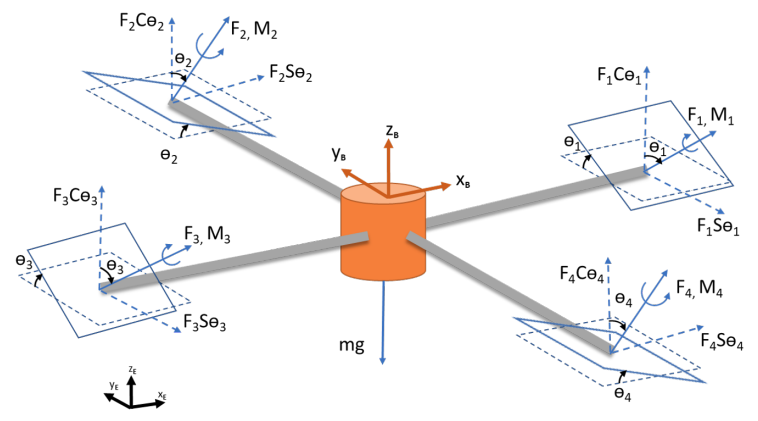
\includegraphics[width=0.7\linewidth]{Images/image34.png}
        \caption{Tilting configuration quadcopter.}
    \end{minipage}\hfill
    \begin{minipage}{0.3\textwidth}
        It is now time to introduce UAVs with tilting configurations; the Allocation matrix for a simple quadcopter with tilting configuration can be computed by drawing its free-body diagram:
    \end{minipage}
\end{figure}
\begin{definition}\label{UAV_tilting_allocation_matrix_def}
    The allocation matrix for a tilting configuration quadcopter (\textit{Holocopter method}) is:
    \begin{gather}\label{UAV_tilting_allocation_matrix_Holocopter_approach}
        G_q=
        \begin{bmatrix}
            0 & -k_{f}s_2 & 0 & k_{f}s_4\\
            k_{f}s_1 & 0 & -k_{f}s_3 & 0\\
            -k_{f}c_1 & -k_{f}c_2 & -k_{f}c_3 & -k_{f}c_4\\
            0 & -lk_{f}c_2-k_{m}s_2 & 0 &lk_{f}c_4+k_{m}s_4\\
            lk_{f}c_1+k_{m}s_1 & 0 & -lk_{f}c_3-k_{m}s_3 & 0\\
            lk_{f}c_1-c_mc_1 & -lk_{f}s_2+c_mc_2 & lk_{f}s_3-c_mc_3 & -lk_{f}s_4+c_mc_4
        \end{bmatrix}
    \end{gather}
    With the input vector defined as $u=\begin{bmatrix}
        u_{\omega_1} & u_{\omega_2} & u_{\omega_3} & u_{\omega_4}
    \end{bmatrix}$
\end{definition}
Then, the following geometric model is introduced.
\begin{definition}\label{UAV_tilting_geometric_model_def}
    (\textit{Geometric Model for a tilting quadcopter}): The \textit{Geometric Model} for a tilting configuration UAV is given by:
    \small{
    \begin{gather}\label{UAV_tilting_geometric_model}
        \begin{cases}
            \begin{bmatrix}
                mI_3 & 0 \\ 0 & I_b
            \end{bmatrix}
            \begin{bmatrix}
                \ddot{p}_b\\
                \dot{\omega}_b^b
            \end{bmatrix}=
            \begin{bmatrix}
                mge_3\\
                -S\left(\omega_b^b\right)I_b\omega_b^b
            \end{bmatrix}+
            \begin{bmatrix}
                R_b & 0 \\ 0 & I_3
            \end{bmatrix}
            \begin{bmatrix}
                G_{q,f}(\alpha) & 0\\
                G_{q,\tau}(\alpha) & 0
            \end{bmatrix}
            \begin{bmatrix}
                u_\omega\\ u_\alpha
            \end{bmatrix}\\
            \dot{R}_b=R_bS\left(\omega_b^b\right)\\ 
            \dot{\alpha}=u_\alpha
        \end{cases}
    \end{gather} }                
    Where $G_q(\alpha)=\begin{bmatrix}G_{q,f}(\alpha) \\ G_{q,\tau}(\alpha)\end{bmatrix}$ and $u_\alpha \in \mathbb{R}^4$ is the control input vector for the tilting angles.
\end{definition}
Notice that the allocation matrix in this model is \textit{not} full-rank. This is due to the tilting input $u_\alpha$ acting at a higher differential level than $u_\omega$; therefore a direct dynamics inversion at acceleration level involves only $u_\omega$, resulting in loss of controllability. This implies that, for Feedback Linearization, it is necessary to compute higher order Lie Derivatives until also $u_\alpha$ appears. If this is done, a new model is obtained:
\begin{gather*}
    \begin{cases}
        \begin{bmatrix}
            \ddot{p}_b \\ \ddot{\omega}_b^b
        \end{bmatrix}=b\left(R_b,\omega_b^b,\dot{\omega}_b^b,\alpha,u_\omega \right)+A\left(R_b,\alpha,u_\omega\right)
        \begin{bmatrix}
            u_v\\ u_\alpha
        \end{bmatrix}\\
        \dot{R}_b=R_bS\left(\omega_b^b\right)\\
        \dot{\alpha}=u_\alpha\\
        \dot{u}_\omega=u_v
    \end{cases}\\
    A=
    \begin{bmatrix}
        mI_3 & 0 \\ 0 & I_b
    \end{bmatrix}^{-1}
    \begin{bmatrix}
        R_b & 0 \\ 0 & I_3
    \end{bmatrix}
    \begin{bmatrix}
        G_q(\alpha) & \sum_{i=1}^{4}\frac{\partial g_{q,i}(\alpha)}{\partial\alpha}u_{\omega_i}
    \end{bmatrix}
\end{gather*}
Notice how $A\in\mathbb{R}^{6 \times 8}$ has full-rank as long as $u_\omega\neq0$, meaning until the propellers don't all stop. If the task is to track the desired position, velocity, and acceleration for the translational and angular part, a classic PID controller plus jerk feed-forward can be employed; since the system is redundant with respect to the given task, it is possible to employ the redundancy to optimize additional criteria (e.g., minimizing the norm of $u_\omega$ for energy consumption).\\
However, it would be easier on the life of the designer if it was possible to directly design the input forces and torques. There is a way to do this, by redefining the allocation matrix as:
\begin{definition}\label{UAV_tilting_allocation_matrix_Voliro_approach_def}
    The modified allocation matrix (\textit{Voliro approach}) for a tilting quadcopter is given by:
    \begin{gather}\label{UAV_tilting_allocation_matrix_Voliro_approach}
        G_q=
        \begin{bmatrix}
            0 & 0 & 0 & -1 & 0 & 0 & 0 &1\\
            0 & 1 & 0 & 0 & 0 & -1 & 0 & 0\\
            -1 & 0 & -1 & 0 & -1 & 0 & -1 & 0\\
            0 & 0 & -l & -k_{m}/k_{f} & 0 & 0 & l & k_{m}/k_{f} \\
            l & k_{m}/k_{f} & 0 & 0 & -l & -k_{m}/k_{f} & 0 & 0\\
            -k_{m}/k_{f} & l & k_{m}/k_{f} & -l & -k_{m}/k_{f} & l & k_{m}/k_{f} & -l
        \end{bmatrix}
    \end{gather}
    The control input to this system $u(\alpha,u_\omega)$ is defined as:
    \begin{equation*}
        u(\alpha,u_\omega)=
        \begin{bmatrix}
            u_{v,1} & u_{l,1} & u_{v,2} & u_{l,2} & u_{v,3} & u_{l,3} & u_{v,4} & u_{l,4}
        \end{bmatrix}^{T}
    \end{equation*}
    Where $u_{v,i}=k_{f} u_{\omega_i} c_{\theta_i}$, $u_{l,i}=k_{f} u_{\omega_i} s_{\theta_i}$ for $i\in\{1,\dots,4\}$.
\end{definition}
This gives the modified model:
\begin{definition}\label{UAV_tilting_model_modified_def}
    The allocation matrix defined previously results in the modified model:
    \begin{equation}\label{UAV_tilting_model_modified}
        \begin{cases}
            m\ddot{p}_b=mge_3+R_bf^b\\
            \dot{R}_b=R_bS\left(\omega_b^b\right)\\
            I_b\dot{\omega}_b^b=-S\left(\omega_b^b\right)I_b\omega_b^b+\tau^b
        \end{cases}
    \end{equation}
\end{definition}
The inputs $f^b,\tau^b$ are then obtained by pseudo-invertion of the allocation matrix:
\begin{gather*}
    \begin{cases}
        u_{\omega_i}=\frac{1}{k_{f}}\sqrt{u_{l,i}^{2}+u_{v,i}^2}\\
        \alpha_i=atan2(u_{l,i},u_{v,i})        
    \end{cases}\\
    i\in\{1,\dots,4\}
\end{gather*}
However there are two major drawbacks to this approach:
\begin{itemize}
    \item Allocating the actuator commands using the pseudoinverse may result in inadmissible rotor speeds that are higher than physically possible.
    \item This allocation does not account for the slower dynamics of the tilting angles, which leads to forces and moments being produced in directions that have not been commanded.
\end{itemize}
\subsection{Dynamic Models: Unmanned Aerial Manipulator}
An \textit{Unmanned Aerial Manipulator} is just an UAV with a manipulator mounted on it. To model its dynamics, let us define the vector of generalized joint vector:
\begin{gather*}
    \zeta=\begin{bmatrix}
        p_{b} & \eta_{b} & q_{1} & \dots & q_{n}
    \end{bmatrix}^{T}\in\mathbb{R}^{6+n}
\end{gather*}
As usual, the robot's kinematics is referred to the world frame by the homogeneous transformation matrix:
\begin{gather*}
    T_{e}=T_{b}T_{e}^{b}, \text{  }T_{e}\in SE(3)=\mathbb{R}^{3}\times SO(3)
\end{gather*}
Where $T_{b}$ is the transformation describing the robot's pose with respect to the world frame and $T_{e}^{b}$ the one describing the end-effector's pose with respect to the body frame. The kinematics is then given by differentiation:
\begin{gather*}
    \begin{bmatrix}
        \dot{p}_{b} \\ \omega_{b}^{b} \\ \dot{p}_{e}^{b} \\ \omega_{e}^{b}
    \end{bmatrix}=
    \begin{bmatrix}
        I_{3} & 0_{3} & 0\\
        0_{3} & Q(\eta_{b}) & 0\\
        0 & 0 & J(q)
    \end{bmatrix}
\end{gather*}
Define for each link a local reference frame attached to its Center of Mass, similarly as has been done previously in the context of robotic manipulators; each CoM position is then given as:
\begin{gather*}
    p_{l_{i}}=p_{b}+R_{b}p_{b_{l_{i}}}^{b}, \text{ }i=1,\dots,n
\end{gather*}
Where $p_{b_{l_{i}}}^{b}$ is the link's CoM position with respect to the body frame. Since the generalised velocities of each link can be expressed by Jacobians and the generalised joint velocities such as:
\begin{gather*}
    \dot{p}_{b_{l_{i}}}=J_{p}^{(l_{i})}\dot{q}\\
    \omega_{b_{l_{i}}}=J_{o}^{(l_{i})}\dot{q}
\end{gather*}
The link's velocities in the World Frame are:
\begin{gather*}
    \dot{p}_{b_{l_{i}}}=\dot{p}_{b}-S\left(R_{b}p_{b_{l_{i}}}\right)\omega_{b}+R_{b}J_{p}^{(l_{i})}\dot{q}\\
    \omega_{l_{i}}=\omega_{b}-R_{b}J_{o}^{(l_{i})}\dot{q}
\end{gather*}
These are used in the Lagrangian Formalism to get the model:
\begin{gather*}
    B(\zeta)\ddot{\zeta}+C(\zeta,\dot{\zeta})\dot{\zeta}+\bar{g}(\zeta)=u
\end{gather*}
With the usual meanings for the symbols. The system's input, in the cae of a flat configuration UAV and a fully-actuated manipulator, is:
\begin{gather*}
    f=
    \begin{bmatrix}
        u_{T} & \tau^{b} & \tau_{q}
    \end{bmatrix}^{T}\in\mathbb{R}^{4+n}
\end{gather*}
Where $\tau_q\in\mathbb{R}^{n}$ are the manipulator's torques. The relationship between $u$ and $f$ is not immediate, and is given by:
\begin{gather*}
    u=diag\{R_{b}e_{3},Q^{T},I_{n}\}=\Omega f\\
    \Omega\in\mathbb{R}^{(n+6)\times(n+4)}
\end{gather*}
The control of such a system will not be part of the discussion here, however there are mainly two approaches: centralized and decentralized control. The first, which is especially useful in the case of non-tilting configurations (which are underactuated), it to directly compute the input for all propellers and the manipulator, so that the UAV and manipulator dynamics are coupled; in the case of decentralized control, the two dynamics are thought of as uncoupled.
\section{Control and Flat Outputs}
\subsection{Flat Outputs}
The quadrotor is a differentially flat system, with flat outputs $(x,y,z,\psi)$; this means that the UAV trajectory can be planned as a function of the flat outputs; still, due to the UAV's underactuation (in the case of non-tilting configurations), it is impossible to controll the full pose. \\
Let us consider the RPY model eq:\ref{UAV_RPY_compact_model}, for which the state is chosen to be $x=[\zeta,\dot{\zeta}]^{T}$; then, the diffeomorphism $\sigma:\mathbb{R}^n\rightarrow\mathbb{R}^n$ linking the state to the flat outputs is given by:
\begin{equation}\label{UAV_flat_outputs}
    \sigma=
    \begin{bmatrix}
        \sigma_1 \\ \sigma_2 \\ \sigma_3 \\ \sigma_4
    \end{bmatrix}=
    \begin{bmatrix}
        x \\ y \\ z \\ \psi
    \end{bmatrix}
\end{equation}
Its inverse is given as:
\begin{equation}\label{UAV_state_from_flat_outputs}
    \begin{cases}
        x=\sigma_1\\
        y=\sigma_2\\
        z=\sigma_3\\
        \phi=\sin^{-1}\left(\frac{\ddot{\sigma}_{2}\cos(\sigma_4)-\ddot{\sigma}_{1}\sin(\sigma_4)}{\sqrt{\ddot{\sigma}_{1}^{2}+\ddot{\sigma}_{2}^{2}+\left(\ddot{\sigma}_{3}-g\right)^{2}}}\right) \\
        \theta=\tan^{-1}\left(  \frac{\ddot{\sigma}_{1}\cos(\sigma_4)+\ddot{\sigma}_{2}\sin(\sigma_4)}{\ddot{\sigma}_3-g} \right)\\
        \psi=\sigma_4
    \end{cases}
\end{equation}
The inputs to the system then should be:
\begin{gather}\label{UAV_flat_outputs_inputs}
    \begin{cases}
        u_{T}=m\sqrt{\ddot{\sigma}_{1}^{2}+\ddot{\sigma}_{2}^{2}+\left(\ddot{\sigma}_{3}-g\right)^{2}} \\
        \tau_{b}^{b}=J_{b}\left[\dot{R}_{b}^{T}+R_{b}^{T}\ddot{R}_{b}\right]^{\vee}+R_{b}^{T}\dot{R}_{b}J_{b}\left[R_{b}^{T}\dot{R}_{b}\right]^{\vee}
    \end{cases}
\end{gather}
Where $\vee$ is the \textit{Vee-operator}, i.e. the inverse of the skew-symmetric operator. Notice that the inputs include the dynamics, which means that these inputs are only allowed if feed-forward control is sufficient.
\subsection{Hierarchical Controller of a Quadcopter}
Starting from the RPY model of eq:\ref{UAV_RPY_dyn_model}, ignoring external disturbances, it is possible to design a type of \textit{Hierarchical Controller}; its main structure is:
\begin{itemize}
    \item A linear subsystem, concerning the quadcopter's linear dynamics.
    \item A linear subsystem, concerning the quadcopter's angular dynamics.
    \item A nonlinear interconnection between the subsystems.
\end{itemize}
To this end, a feedback linearization is carried out on the angular dynamics, by the input:
\begin{equation*}
    \tau^b=J_{b}Q(\eta_b)\tilde{\tau}+Q(\eta_b)^{-T}C(\eta_b,\dot{\eta}_b)\dot{\eta}_b
\end{equation*}
Notice that there is a singularity at $\theta=\pm\pi/2$, which is not a surprise since the Euler Angles are involved in this model. Define the attitude error $e_\eta$:
\begin{gather}\label{UAV_hier_attitude_error}
    e_\eta=
    \begin{bmatrix}
        e_\phi \\ e_\theta \\ e_\psi
    \end{bmatrix}=
    \eta_n-\eta_{b,d}=
    \begin{bmatrix}
        \phi \\ \theta \\ \psi
    \end{bmatrix} -
    \begin{bmatrix}
        \phi_d \\ \theta_d \\ \psi_d
    \end{bmatrix} 
\end{gather}
The quadcopter model then becomes\footnote{Notice that in the error definition it is assumed that a desired orientation is known, although it is not controllable. This would seem a contradiction, but remember that the quadcopter is a flat system: the desired attitude can be computed by the flat outputs.
\begin{gather*}
    \varphi_d=\sin^{-1}\left[\frac{m}{u_T}\left(\cos(\psi_d)-\mu_x\sin(\psi_d)\right)\right] \\
    \theta_d=\tan^{-1}\left[\frac{\mu_x\cos(\psi_d)+\mu_y\sin(\psi_d)}{\mu_z-g}\right]
\end{gather*}
Notice the singularity for $\mu_z=g$; the planner should avoid this by committing to the constraint $|\mu_z|<g$.
}:
\begin{gather*}
    \begin{cases}
        \ddot{p}_b=\left\{-\frac{1}{m}u_{T}R_b(\eta_{b,d})e_3+ge_3\right\}+\frac{1}{m}u_{T}\delta(\eta_{b,d},\eta_{n})\\
        \ddot{\eta}_b=\tilde{\tau}\\
        \delta(\eta_{b,d},e_\eta)=
        \begin{bmatrix}
            s_{\phi_d}s_{\psi_d}-s_{\phi}s_{\psi}-c_{\phi}c_{\psi}s_{\theta}+c_{\phi_d}c_{\psi_d}s_{\theta_d}\\
            c_{\psi}s_{\theta}-s_{\phi_d}c_{\psi_d}+c_{\phi_d}s_{\psi_d}s_{\theta_d}-c_{\phi}c_{\psi}s_{\theta}\\
            c_{\phi_d}c_{\theta_d}-c_{\phi}c_{\theta}
        \end{bmatrix}
    \end{cases}
\end{gather*}
Resulting in:
\begin{equation}\label{UAV_hierachical_interconnection_model}
    \begin{cases}
        \ddot{p}_b=\mu_d+\frac{1}{m}u_{T}\delta(\eta_{b,d},\eta_{n})\\
        \ddot{\eta}_b=\tilde{\tau}\\
        \delta(\eta_{b,d},e_\eta)=
        \begin{bmatrix}
            s_{\phi_d}s_{\psi_d}-s_{\phi}s_{\psi}-c_{\phi}c_{\psi}s_{\theta}+c_{\phi_d}c_{\psi_d}s_{\theta_d}\\
            c_{\psi}s_{\theta}-s_{\phi_d}c_{\psi_d}+c_{\phi_d}s_{\psi_d}s_{\theta_d}-c_{\phi}c_{\psi}s_{\theta}\\
            c_{\phi_d}c_{\theta_d}-c_{\phi}c_{\theta}
        \end{bmatrix}
    \end{cases}
\end{equation}
Where $\delta(\eta_{b,d},e_\eta)$ is the nonlinear connection between the two linear subsystems mentioned earlier. The error dynamics are easily found from the linearized system:
\begin{gather*}
    \begin{cases}
        \begin{bmatrix}
            \dot{e}_p \\ \ddot{e}_p
        \end{bmatrix}=
        \begin{bmatrix}
            0 & I \\ 0 & 0
        \end{bmatrix}
        \begin{bmatrix}
            e_p \\ \dot{e}_p
        \end{bmatrix}+
        \begin{bmatrix}
            0 \\ I
        \end{bmatrix}
        \left(\mu_d-\ddot{p}_{b,d}\right)+\frac{1}{m}u_{T}
        \begin{bmatrix}
            0 \\ \delta(\eta_{b,d},e_\eta)
        \end{bmatrix}\\
        \begin{bmatrix}
            \dot{e}_\eta \\ \ddot{e}_\eta
        \end{bmatrix}=
        \begin{bmatrix}
            0 & I \\ 0 & 0
        \end{bmatrix}
        \begin{bmatrix}
            e_\eta \\ \dot{e}_\eta
        \end{bmatrix}+
        \begin{bmatrix}
            0 \\ I
        \end{bmatrix}
        \left(\tilde{\tau}-\ddot{\eta}_{b,d}\right)
    \end{cases} \rightarrow \\
    \begin{cases}
        \begin{bmatrix}
            \dot{e}_p \\ \ddot{e}_p
        \end{bmatrix}=A
        \begin{bmatrix}
            e_p \\ \dot{e}_p
        \end{bmatrix}+B
        \left(\mu_d-\ddot{p}_{b,d}\right)+\frac{1}{m}u_{T}
        \Delta\\
        \begin{bmatrix}
            \dot{e}_\eta \\ \ddot{e}_\eta
        \end{bmatrix}=A
        \begin{bmatrix}
            e_\eta \\ \dot{e}_\eta
        \end{bmatrix}+B
        \left(\tilde{\tau}-\ddot{\eta}_{b,d}\right)
    \end{cases}
\end{gather*}
The system can be stabilized by the simple controller:
\begin{gather*}
    \begin{cases}
        \mu_d=-K_p
        \begin{bmatrix}
            e_p \\ \dot{e}_p
        \end{bmatrix} + \ddot{p}_{b,d}\\
        \tilde{\tau}=-K_{e}
        \begin{bmatrix}
            e_\eta \\ \dot{e}_\eta
        \end{bmatrix}+\ddot{\eta}_{b,d}
    \end{cases}
\end{gather*}
With $K_p,K_e\in\mathbb{R}^{3\times 6}$ are chosen such that $A_p=A-BK_p, A_e=A-BK_e$ are Hurwitz. The resulting closed-loop system is asymptotically stable, however the asymptotically stability of the interconnection requires the use of perturbation theory and will not be addressed here. 
\begin{gather*}
    \begin{cases}
        \begin{bmatrix}
            \dot{e}_p \\ \ddot{e}_p
        \end{bmatrix}=A
        \begin{bmatrix}
            e_p \\ \dot{e}_p
        \end{bmatrix}+\frac{1}{m}u_{T}\Delta\\
        \begin{bmatrix}
            \dot{e}_\eta \\ \ddot{e}_\eta
        \end{bmatrix}=A_e
        \begin{bmatrix}
            e_\eta \\ \dot{e}_\eta
        \end{bmatrix}
    \end{cases}
\end{gather*}
In conclusion, a Hierarchical Controller is composed by:
\begin{itemize}
    \item An outer loop: given the desired linear position, velocity, and acceleration from the planner, it is possible to compute:
    \begin{equation*}
        \mu_d =
        \begin{bmatrix}
            e_p \\ \dot{e}_p
        \end{bmatrix}+\ddot{p}_{b,d}
    \end{equation*}
    Then, we find the total thrust and the reference for the roll and the pitch angles.
    \item An inner loop: once having computed the desired attitude by the flat outputs, a second-order filter is used to obtain the necessary derivatives; then $\tilde{\tau},\tau$ are computed from the linearizing feedback input formula. Then, the propellers' velocities are assigned.
\end{itemize}
\subsection{\textit{Geometric Controller} of a Quadcopter}
Consider the coordinate-free geometrical model of eq:\ref{UAV_geomtric_dyn_model}. In a geometrical controller the main objective is two-fold:
\begin{itemize}
    \item Align the body $z$-axis with a desired axis.
    \item Choose the appropriate $u_T$ to follow the desired trajectory.
\end{itemize}
This is done by appropriately choosing $u_T$ and more importantly $R_{b,d}e_3$: this last choice is critical, in the sense that it could happen that the triplet $(x_{b,d},y_{b,d},z_{b,d})$ is not mutually orthogonal. To avoid this, a projection operation is executed, defining then $R_{b,d}$ as:
\begin{equation}\label{UAV_geometric_control_desired_z}
    R_{b,d}=
    \begin{bmatrix}
        S(y_{b,d}) & \frac{S(z_{b,d})x_{b,d}}{||S(z_{b,d})x_{b,d}||} & z_{b,d}
    \end{bmatrix}
\end{equation}
Also, to ensure that the planned desired linear acceleration does not exceed $g$, assume that $||-mge_3+m\ddot{p}_{b,d}||<M$, where $M>0$.
Define the errors:
\begin{gather}\label{UAV_geometric_controller_errors}
    e_p=p_b-p_{b,d}\\
    e_{R}=\frac{1}{2}\left[R_{b,d}^{T}R_{b}-R_{b}^{T}R_{b,d}\right]^{\vee}\\
    e_{\omega}=\omega_{b}^{b}-R_{b}^{T}R_{b,d}\omega_{b,d}^{b,d}
\end{gather}
Then, the control system is composed by:
\begin{itemize}
    \item An outer-loop control, defined by:
    \begin{gather}\label{UAV_geometric_controller_outer_loop_u}
        u_{T}=-\left[-K_pe_p-K_v\dot{e}_p-mge_3+m\ddot{p}_{b,d}\right]^{T}R_be_3\\
        z_{b,d}=-\frac{-K_pe_p-K_v\dot{e}_p-mge_3+m\ddot{p}_{b,d}}{||-K_pe_p-K_v\dot{e}_p-mge_3+m\ddot{p}_{b,d}||}
    \end{gather}
    \item An inner-loop control, defined by:
    \begin{gather*}
        \tau^b=-K_Re_R-K_{\omega}e_{\omega}+S\left(\omega_{b}^{b}\right)I_b\omega_{b}^{b}-I_b\left[ S\left(\omega_{b}^{b}\right)R_{b}^{T}R_{b,d}\omega_{b,d}^{b,d}-R_{b}^{T}R_{b,d}\dot{\omega}_{b,d}^{b,d} \right]
    \end{gather*}
\end{itemize}
Under this control the closed-loop dynamics becomes:
\begin{equation*}
    m\ddot{e}_p+K_v\dot{e}_p+K_pe_p=-\frac{u_T}{e_3^TR_{b,d}^TR_be_3}\left[\left(e_3^TR_{b,d}^TR_be_3\right)R_be_3-R_{b,d}e_3\right]
\end{equation*}
Notice that the RHS plays the role of the interconnection term,  as already seen in the previous section on Hierarchial Control, which becomes zero when the error orientation is null. It is possible to prove exponential stability of the origin by means of Lyapunov Theory.
\subsection{Estimar-Based Control of a quadcopter}
Once again let us consider the RPY model of eq:\ref{UAV_RPY_dyn_model}, this time without neglecting the external disturbances. Define the generalised momentum vector:
\begin{gather}\label{UAV_estimator_based_control_gen_momentum}
    q=
    \begin{bmatrix}
        mI_3 & 0_3\\ 0_3 & M(\eta_b)
    \end{bmatrix}
    \begin{bmatrix}
        \dot{p}_b\\ \dot{\eta}_b
    \end{bmatrix}\rightarrow\\
    \dot{q}=
    \begin{bmatrix}
        mge_3-u_{T}R_be_3+f_e\\
        C^{T}(\eta_b,\dot{\eta}_b)\dot{\eta}_b+Q^{T}(\eta_b)\tau^{b}+\tau_e
    \end{bmatrix}
\end{gather}
The estimator's job is to estimate the external wrench $[f_e,\tau_e]$. For simplicity, assume a linear relationship between the external wrench and its estimation in the Laplace domain:
\begin{equation*}
    \mathcal{L}
    \begin{bmatrix}
        \begin{bmatrix}
            \hat{f}_e \\ \hat{\tau}_e
        \end{bmatrix}    
    \end{bmatrix}=
    G(s)\mathcal{L}
    \begin{bmatrix}
        \begin{bmatrix}
            f_e \\ \tau_e
        \end{bmatrix}    
    \end{bmatrix}
\end{equation*}
Where $G(s)=diag(\{G_i(s)\})$, $i\in\{1,\dots,6\}$. To further simplify, let:
\begin{equation*}
    G_i(s)=\frac{k_0}{s+c_0}, i\in\{1,\dots,6\}
\end{equation*}
The choice of the gains $k_0,c_0>0$ is critical; an obvious choice is $k_0=c_0$, which doesn't give any amplification during the estimation. Assume that the estimator is turned-on before the UAV's take-off and applying the inverse Laplace transform:
\begin{gather*}
    \frac{d}{dt}
    \begin{bmatrix}
        \hat{f}_e \\ \hat{\tau}_e    
    \end{bmatrix}=k_0 
    \begin{bmatrix}
        f_e(t) \\ \tau_e(t)
    \end{bmatrix}-
    \begin{bmatrix}
        \hat{f}_e(t) \\ \hat{\tau}_e(t)
    \end{bmatrix}\rightarrow\\
    \frac{d}{dt}
    \begin{bmatrix}
        \hat{f}_e \\ \hat{\tau}_e    
    \end{bmatrix}=k_0
    \left\{
    \dot{q}-
    \begin{bmatrix}
        mge_3-u_{T}R_be_3 \\ C^{T}(\eta_b,\dot{\eta}_b)\dot{\eta}_b+Q^{T}(\eta_b)\tau^b
    \end{bmatrix}
    \right\}-
    \begin{bmatrix}
        \hat{f}_e(t) \\ \hat{\tau}_e(t)
    \end{bmatrix}\rightarrow\\
    \begin{bmatrix}
        \hat{f}_e \\ \hat{\tau}_e    
    \end{bmatrix}=k_0
    \left\{
    \dot{q}-
    \int_{0}^{t}\left\{
    \begin{bmatrix}
        mge_3-u_{T}R_be_3 \\ C^{T}(\eta_b,\dot{\eta}_b)\dot{\eta}_b+Q^{T}(\eta_b)\tau^b
    \end{bmatrix}
    -
    \begin{bmatrix}
        \hat{f}_e(t) \\ \hat{\tau}_e(t)
    \end{bmatrix}
    dt \right\}
    \right\}
\end{gather*}
Notice that to correctly estimate the external wrench it is needed to measure:
\begin{itemize}
    \item The UAV's attitude (IMU sensor).
    \item The UAV's angular velocity (IMU sensor).
    \item The UAV's linear velocity (GPS/On-board devices).
    \item The UAV's inputs (the controller gives these directly).
    \item The UAV's model's parameters.
\end{itemize}
Obviously, higher order filters can be employed; as an example, the same procedure just outlined could be replicated with a $r$-th order estimator:
\begin{equation*}
    G_i(s)=\frac{c_0}{s^r+c_{r-1}s^{r-1}+\dots+c_1s+c_0}
\end{equation*}
Building the Hurwitz Polynomial and then the filter:
\begin{gather*}
    \sum_{i=0}^{r} \prod_{j=-r}^{-(i+1)}{K_j\frac{d^i}{dt^i}
    \begin{bmatrix}
        \hat{f}_e(t) \\ \hat{\tau}_e(t)    
    \end{bmatrix}}=
    \prod_{i=1}^{r}K_i 
    \begin{bmatrix}
        f_e(t) \\ tau_e(t)
    \end{bmatrix}\\
    \gamma_1(t)=K_1\left\{q-\int_{0}^{t}\left\{
    \begin{bmatrix}
        \hat{f}_e \\ \hat{\tau}_e
    \end{bmatrix}+
    \begin{bmatrix}
        mge_3-u_{T}R_be_3\\
        C^{T}(\eta_b,\dot{\eta}_b)\dot{\eta}_b+Q^{T}(\eta_b)\tau^b
    \end{bmatrix}
    \right\}dt
    \right\}\\
    \gamma_i(t)=K_i \int_{0}^{t}\left\{
    -\begin{bmatrix}
        \hat{f}_e\\ \hat{\tau}_e
    \end{bmatrix}+\gamma_{i-1}
    \right\}dt, i=2,\dots,r\\
    \prod_{i=j+1}^{r}K_i=c_j,j=0,\dots,r-1
\end{gather*}
\subsection{Passivity-Based Controller with Compensation of external wrench}
Let us consider once again the RPY model of a quadcopter of e1:\ref{UAV_RPY_dyn_model}. In the previous sections, the use of feedback linearization and an estimator have been illustrated. However, one of the (if not "the") flaws of I/O Feedback Linearization is its reliance of a perfect model for the UAV, although it is obviously not generally the case that a perfect model is available. If I/L FL is to be avoided, an alternative is represented by \textit{Passive Control}. In this section both a Passivity-Based Controller and the Estimator discussed in the previous section will be employed.\\
Let us design an inner/outer-loop controller; for the inner-loop define:
\begin{itemize}
    \item $\dot{\eta}_b=\dot{\eta}_{b,d}-\sigma e_\eta$, where $\sigma>0$ is a coupling parameter.
    \item $\ddot{\eta}_{r}=\ddot{\eta}_{b,d}-v\dot{e}_\eta$.
    \item $e_\eta=\eta_b-\eta_{b,d}$.
    \item $\dot{e}_\eta=\dot{\eta}_b-\dot{\eta}_{b,d}$.
    \item $v_\eta=\dot{e}_\eta+\sigma e_\eta$
\end{itemize}
Then, the control input:
\begin{gather*}
    \tau^b=Q^{-T}\left[ M(\eta_{b})\ddot{\eta}_{r}+C(\eta_b.\dot{\eta}_b)\dot{\eta}_r-\hat{\tau}_e-D_0v_\eta-K_0e_\eta \right]\\
    D_0,K_0\in\mathbb{R}^{3 \times 3}: D_0>0,K_0>0
\end{gather*}
Which will regulate the quadcopter's angular dynamics. For the outer-loop, define the errors:
\begin{itemize}
    \item $e_p=p_b-p_{b,d}$.
    \item $\dot{e}_p=\dot{p}_b-\dot{p}_{b,d}$.
    \item $\ddot{e}_p=\ddot{p}_b-\ddot{p}_{b,d}$.
    \item $\mu_d=(1/m)\left[ge_3+\hat{f}_e-u_{T}R_b(\eta_{b,d})e_3\right]$.
    \item $\tilde{f}=f_e-\hat{f}_e$, the linear estimation error.
\end{itemize}
Then, by substitution of $\eta_b=e_\eta+\eta_{b,d}$ the linear dynamics becomes:
\begin{equation*}
    \ddot{p}_b=\mu_d+\frac{1}{m}\left[\delta\cdot u_{T}+\tilde{f}\right]
\end{equation*}
Where $\delta$ is the interconnection term that was described in equations eq:\ref{UAV_hierachical_interconnection_model}; also, as in the Hierachical Control method, neglecting for a moment the underactuation of the quadcopter (remembering that the desired attitude can be however computed), define:
\begin{equation*}
    \mu_d=-K_d\dot{e}_p-K_pe_p+\ddot{p}_{b,d}
\end{equation*}
The closed-loop dynamics becomes:
\begin{gather}\label{UAV_passivity_control_closed_loop}
    m\ddot{e}_p+K_d\dot{e}_p+K_pe_p=u_{T}\delta+\tilde{f}\\
    M\dot{v}_\eta+\left(C+D_0\right)v_\eta+K_0e_\eta=\tilde{\tau}
\end{gather}
Both closed-loop equations can be seen as mass-damping-spring systems with programmable stiffness, partially-programmable damping and given mass and inertia; also, notice that:
\begin{itemize}
    \item $K_p,K_d$ have physical meanings, which is always of help for the designer.
    \item The linear part is slower than the angular one, meaning that the closed-loop linear dynamics is defined and the estimator's bandwidth can be exactly tuned to be faster that it.
    \item The coupling factor $\sigma$ should be properly tuned since it affects the tracking results dramatically; in fact, for small values of $\sigma$ the robot could start to vibrate. A common choice is $K_0=\sigma D_0$ (which is equivalent to writing a quadratic optimization problem).
\end{itemize}
Then, the total thrust can be computed from the desired acceleration vector as usual:
\begin{gather*}
    \bar{\mu}=\begin{bmatrix}
        \bar{\mu}_{x} & \bar{\mu}_{y} & \bar{\mu}_{z}
    \end{bmatrix}=
    \mu_{d}-\frac{1}{m}\hat{f}_{e}\\
    u_{T}=m\sqrt{\bar{\mu}^{2}_{x}+\bar{\mu}^{2}_{y}+\left(\bar{\mu}_{z}-g\right)^{2}}\\
    \varphi_{d}=\sin^{-1}\left(\frac{m}{u_{T}}\left[\bar{\mu}_{y}\cos(\psi_{d})-\bar{\mu}_{x}\sin(\psi_{d})\right]\right)\\
    \theta_{d}=\tan^{-1}\left(\frac{\bar{\mu}_{x}\cos(\psi_{d})+\bar{\mu}_{y}\sin(\psi_{d})}{\bar{\mu}_{z}-g}\right)
\end{gather*}
Granted that $\bar{\mu}=\mu_{d}-\frac{1}{m}\hat{f}_{e}=ge_{3}$ should be avoided. The proposed controller can be employed without the estimator of external forces following the same passages for the linear part as for the hierarchical controller.
\section{Disturbance effects}
UAVs (or UAMs) are often employed also in closed environments or have near ground tasks to complete. However, in these situation some disturbance effects arise, due to the environment constricting the propeller's air flows. In this section, some of these effects will be investigated.
\subsection{Ground Effect}
The \textit{Ground Effect} is a disturbance which arises when the UAV is flying close to the ground. The most employed theoretical result for the description of the ground effect is based on the so-called \textit{Potential Aerodynamic Assumption}, which states that the fluid is:
\begin{itemize}
    \item Inviscid.
    \item Incompressible.
    \item Irrotational.
    \item Steady.
\end{itemize}
If these assumptions are satisfied, the \textit{Method of Images}\footnote{The Method of Images is often used also in Electrostatics to compute the polarization of an infinite conducting plane due to the presence of a point-charge placed above it.} can be employed. This method consists in placing a virtual rotor on the opposite side of the ground, which is seen as a barrier, at the same distance from it as the true propeller. 
\begin{figure}[htbp!]
    \centering
    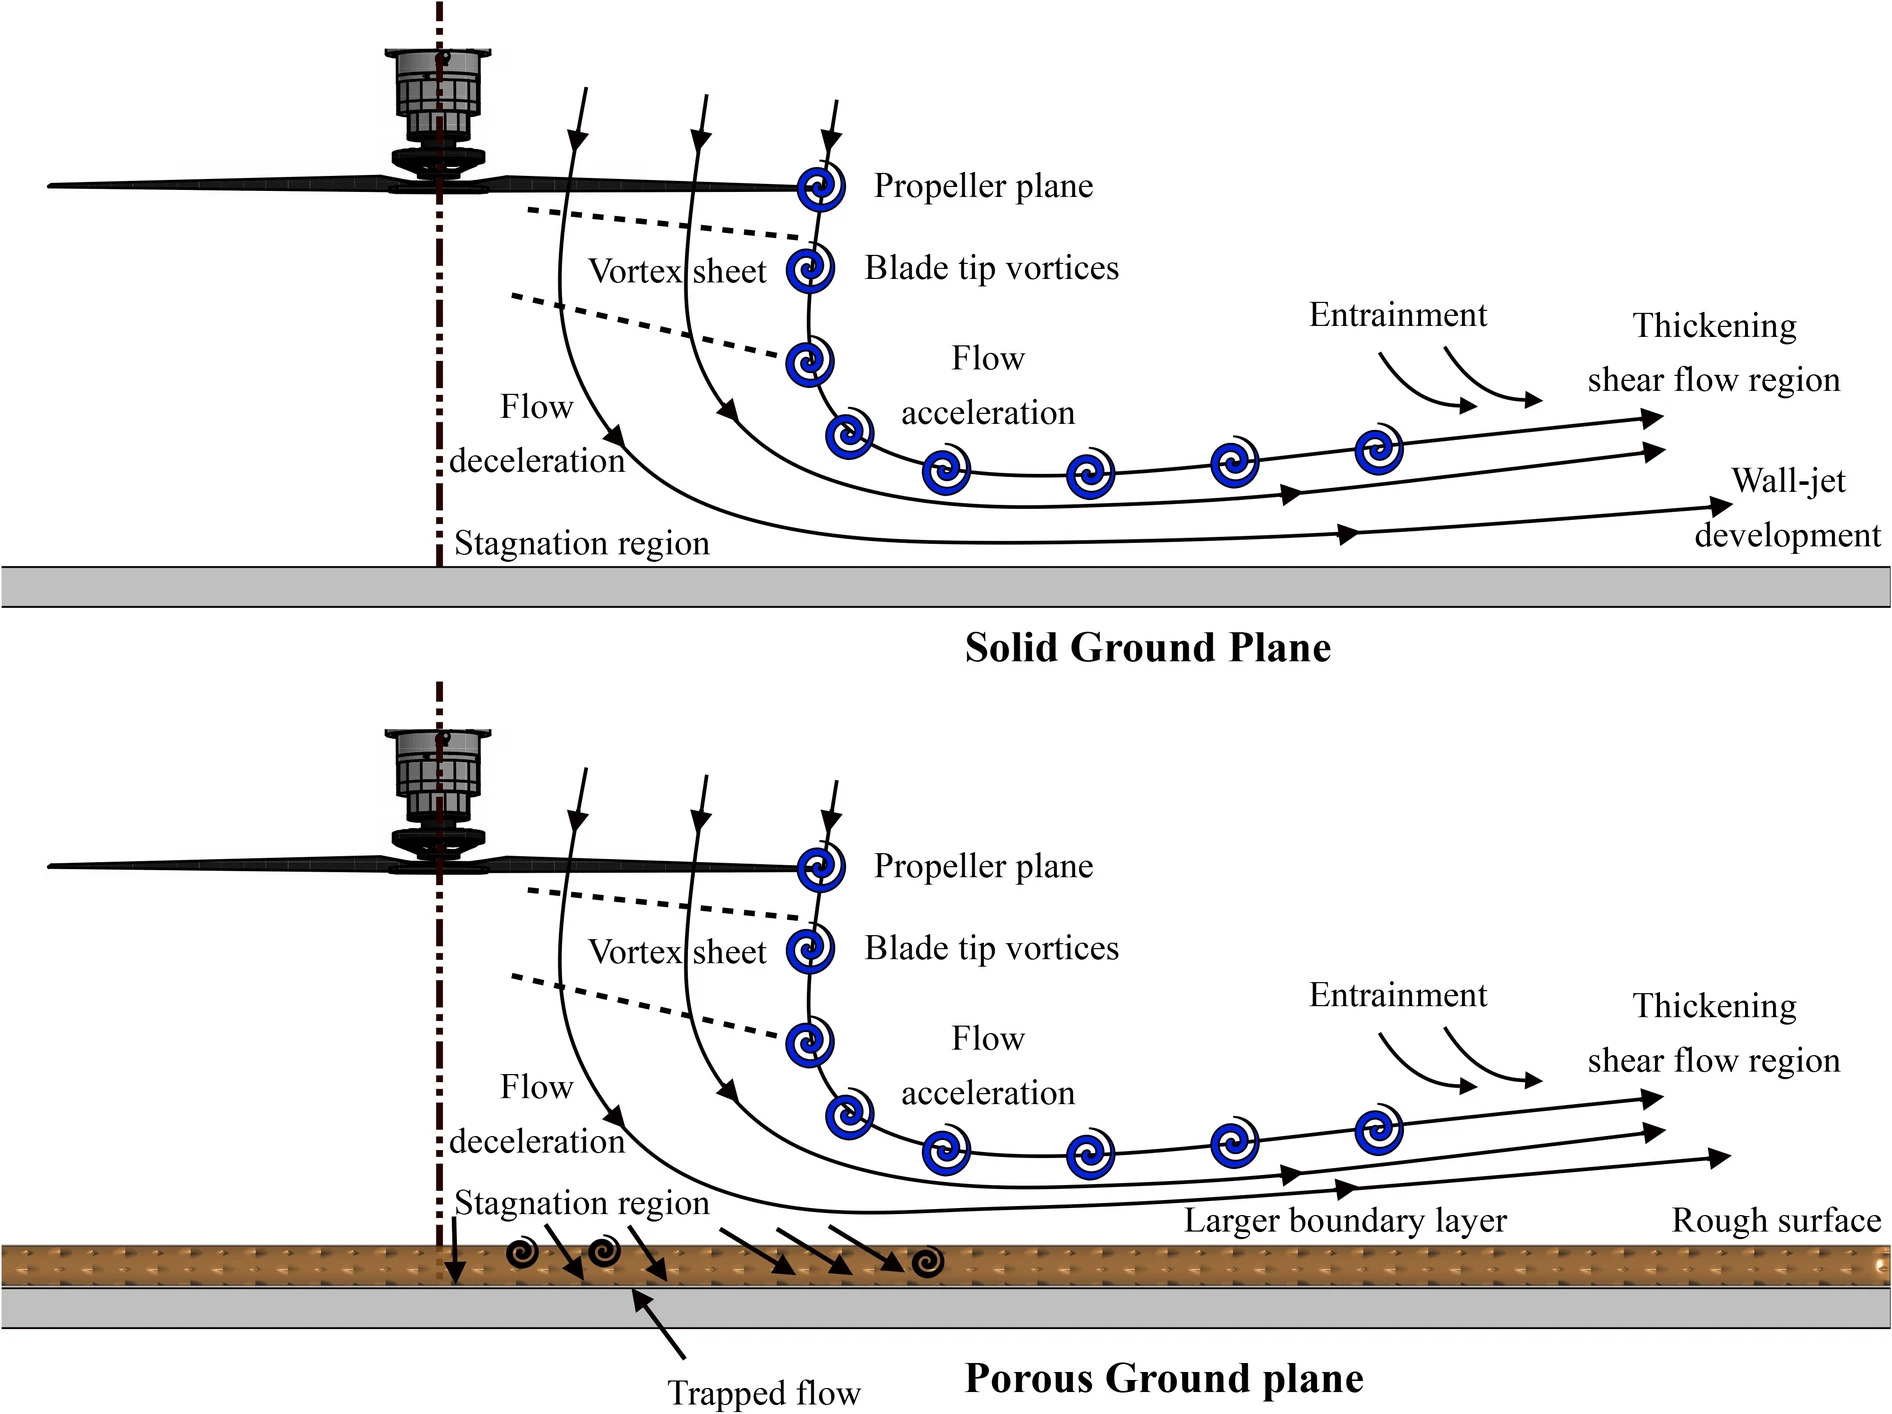
\includegraphics[width=0.6\linewidth]{Images/image35.png}
    \caption{Ground Effect for a single propeller.}
    \label{fig:groud_effect}
\end{figure}\\
Let $v_{IGE},T_{IGE}$ be the induced rotor's velocity and thrust due to the ground effect, respectively. Let $v_{OGE},T_{OGE}$ be the induced rotor's velocity and thrust without ground effect. Then, assuming power conservation between these two situations:
\begin{gather*}
    \frac{T_{IGE}}{T_{OGE}}=\frac{1}{1-\left(\frac{\rho}{4z}\right)^{2}}
\end{gather*}
Where $\rho$ and $z$ are the propeller's radius and height from the ground.
Notice that if $z/\rho=2$ then the formula gives a ratio of $1.016$, meaning that the ground effect for a single propeller is negligible if the propeller is at least two times $\rho$ above ground. The result can be specialized to the case of a quadrotor by simply considering the contributions of each propeller and conservation of power; then:
\begin{gather*}
    \frac{u_{T,IGE}}{u_{T,OGE}}=\frac{1}{1-\left(\frac{\rho}{4z}\right)^{2}-\frac{z\rho^{2}}{\sqrt{\left(d^{2}+4z^{2}\right)^{3}}}-\frac{z\rho^{2}}{2\sqrt{2\left(2d^{2}+4z^{2}\right)^{3}}}}
\end{gather*}
Ground effect causes a net torque around the UAV. This destabilizes the UAV, which tilts and reinforces the Ground effect; this can lead to instability. This is even more annoying in the case of UAMs, which would then rotate away from the object that they are trying to grasp.
\begin{figure}[htbp!]
    \begin{minipage}{0.5\textwidth}
        \centering
        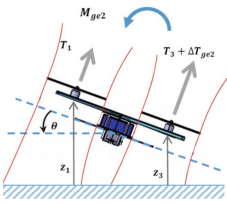
\includegraphics[width=0.6\linewidth]{Images/image36.png}
        \caption{UAV subjected to \\ Ground Effect.}
    \end{minipage}\hfill
    \begin{minipage}{0.5\textwidth}
        \centering
        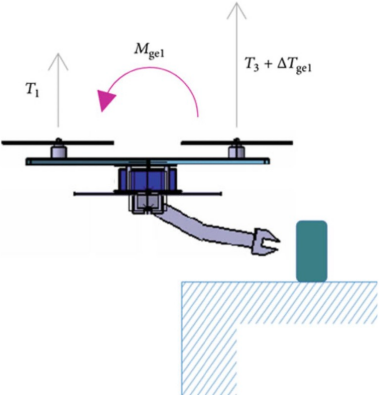
\includegraphics[width=0.5\linewidth]{Images/image37.png}
        \caption{UAM subjected to \\ Ground Effect.}
    \end{minipage} 
\end{figure}
\subsection{Ceiling Effect}
Similar to the Ground Effect, there is also a \textit{Ceiling Effect} which arises when a UAV (or UAM) fly just below a barrier. In the single rotor case, it happens that the thrust increases significantly closes to the ceiling, pushing the rotor even closer to it: this is easily understood by noticing that if the propeller pushes air against the barrier, then a low pressure volume is created above the UAV, which in turn makes the propellers blades spin faster (less air to move out of the way of each blade) increasing its thrust and creating a vacuum (this is called \textit{Vacuum Effect}). Again, this can be mathematically described as:
\begin{gather*}
    \frac{T_{ICE}}{T_{OCE}}=\frac{1}{1-\frac{1}{k_{1}}\left(\frac{\rho}{z+k_{2}}\right)^{2}}
\end{gather*}
Where $T_{ICE},T_{OCE}$ are the thrust with and without Ceiling Effect, respectively; $k_{1}, k_{2}$ are parameters to be tuned. Notice that this effect can be rendered useful by designing the propeller's velocity to make use of the increased thrust, so that a less energy costly and longer flight can be achieved.
\subsection{Wall, Pipe Effects and Flapping Dynamics}
At last, similar to Ground and Ceiling effect, there also exist the so-called \textit{Wall} and \textit{Pipe} effects, whose names are self-explanatory.\\
Much more interesting is the effect of \textit{Flapping Dynamics}, which is an undesirable effect linked to the propeller's blades high rotational velocities. 
\begin{figure}[htbp!]
    \begin{minipage}{0.5\textwidth}
        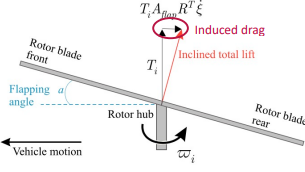
\includegraphics[width=0.75\linewidth]{Images/image38.png}
        \caption{Enter Caption}
    \end{minipage}\hfill
    \begin{minipage}{0.5\textwidth}
        The blades' flapping can be linked to their (however small) elasticity. This flapping causes a different drag force than expected, often neglected since its dissipative nature often actually helps in keeping the UAV stable. However, since each propeller is subjected to these forces, there could be a net torque on the UAV's body, especially during forward motion.
    \end{minipage} 
\end{figure}
Specifically, the advancing rotor blade has a higher velocity then the rear one and it will generate e lift force; in turn, this creates a bigger induced drag than the rear blade resulting in a net force that is opposite to the current forward motion.